\documentclass{article}
\usepackage[margin=1.5cm,bottom=2cm]{geometry}
\usepackage{fancyhdr}
\usepackage{graphicx}
\usepackage{amsmath}
\pagestyle{fancy}

\begin{document}
\fancyhead[L]{ 
\includegraphics[width=2cm]{au_logo.png} }
\fancyhead[R]{CPSC 2320: Computational Physics}
\fancyfoot[C]{\thepage}
\vspace*{0cm}
\begin{center}
	{\LARGE \textbf{Homework 2}}\\
	\vspace{0.25cm}
	{\Large Due: Thursday, October 1}
\end{center}

\section*{Electric field in one dimension}
We want to write a program which will calculate the electric field at a point in space due to a number of electric charges. The charges are all arranged on the X-axis (see the figure). We want the electric field at the origin (x=0).

\begin{figure}[ht!]
	\centering
	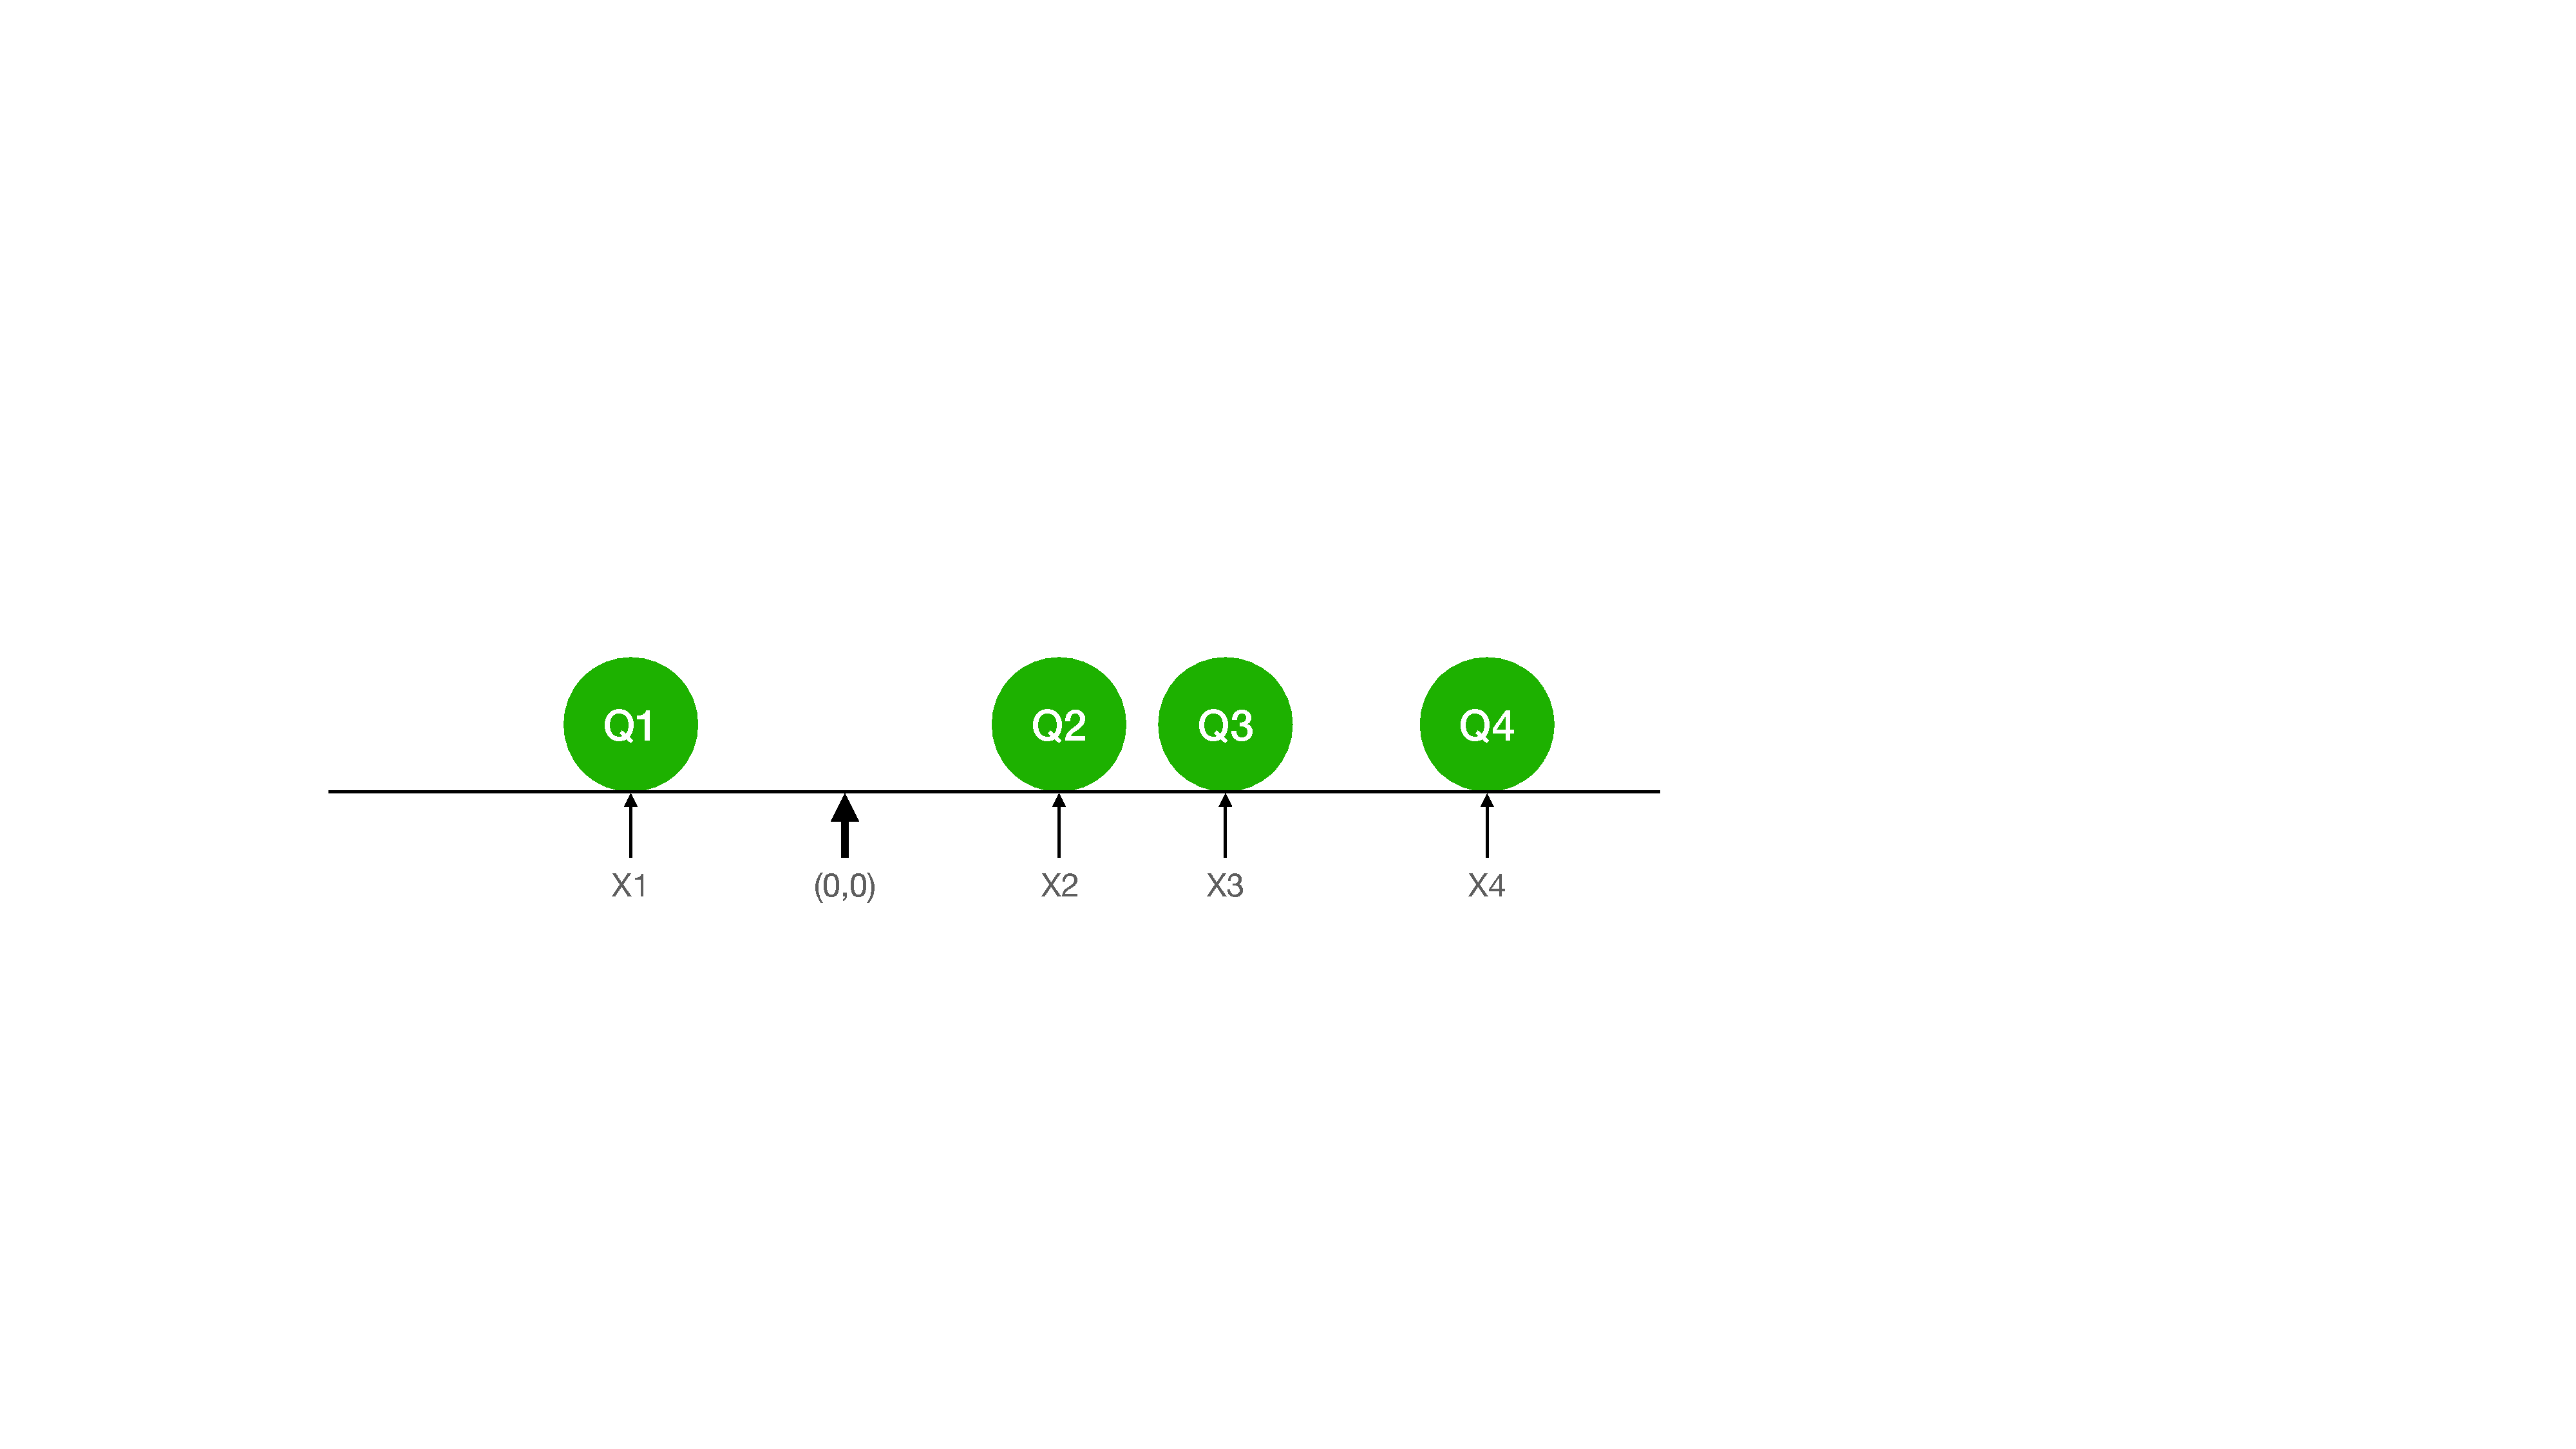
\includegraphics[width=0.6\textwidth]{hw2_sketch}
\end{figure}

Write a C++ program to calculate the electric field of a charge configuration given an array of charges and x positions. Your program should:
\begin{enumerate}
	\item Begin by prompting the user to input the charges (in nano Coulombs) and their positions (in mm). Loop continuously until the user enters a charge value of 0. Do not allow any charges at the origin (x=0).
	
	Example:
	
	\texttt{Please enter values for q and x: -3 5}\\
	\texttt{Please enter values for q and x: 2 4}\\
	\texttt{Please enter values for q and x: 1 0}\\
	\texttt{Cannot place charges at the origin!}\\
	\texttt{Please enter values for q and x: 3 2}\\
	\texttt{Please enter values for q and x: 0 0}\\
	\texttt{Finished looping. Thank you!}
	
	Store these values in two arrays (one for the charge values, one for the position values).  \textit{Hint: In this case you do not know ahead of time how many charges there will be. Declare your array so that you will have enough space, say 100 doubles.}
	
	\item Write a function to calculate the electric field of a single point charge. The equation for this is (given charge q in nC and position x in mm):
	\begin{equation*}
		E = \frac{1}{1000}\frac{kq}{|x|^3}x
	\end{equation*}
	The function should accept $q$ and $x$ as arguments. $k=9\times10^9 \ C^2N^{-1}m^{-2}$ should be declared as a global constant
	
	\item
	The total electric field is the sum of all the individual fields
	\begin{equation*}
		E = \sum_{i=0}^{i=N}E_i=\frac{1}{1000}\frac{kq_0}{x_0^3}x_0 + \frac{1}{1000}\frac{kq_1}{x_1^3}x_1 + \frac{1}{1000}\frac{kq_2}{x_2^3}x_2 + ...
	\end{equation*}
	
	Write a second function which does the following: accept the charge and $x$ arrays as inputs, loop over the arrays and calculate the field of each charge (using the function you wrote earlier) and sum these values. In main(), call this function and print the end result to the user.
\end{enumerate}
\end{document}